\documentclass[12pt]{cdblatex}
\usepackage[final]{pdfpages}
\usepackage{bssn-eqtns}

\begin{document}

\documentclass[12pt]{cdblatex}
\usepackage{bssn-eqtns}

\begin{document}

\section*{PhysRevD.62.044034 equation (9)}

\begin{cadabra}
   from shared import *
   import cdblib

   jsonfile = 'bssn-eqtns-09.json'
   cdblib.create (jsonfile)

   # --------------------------------------------------------------------------

   DgBarDt := \partial_{t}{gBar_{ij}}.           # cdb(eq09.00,DgBarDt)
   DgBarDt := -2 N ABar_{i j}.                   # cdb(eq09.01,DgBarDt)

   canonicalise (DgBarDt)                        # cdb(eq09.02,DgBarDt)  # no change
                                                 # cdb(eq09.99,DgBarDt)  # no change

   cdblib.put ('DgBarDt',DgBarDt,jsonfile)
\end{cadabra}

\begin{dgroup*}
   \begin{dmath*} \cdb{eq09.00} = \Cdb*{eq09.02}\end{dmath*}
\end{dgroup*}

\end{document}

\documentclass[12pt]{cdblatex}
\usepackage{bssn-eqtns}

\begin{document}

\section*{PhysRevD.62.044034 equation (10)}

\begin{cadabra}
   from shared import *
   import cdblib

   jsonfile = 'bssn-eqtns-10.json'
   cdblib.create (jsonfile)

   # --------------------------------------------------------------------------

   DphiDt  := \partial_{t}{\phi}.                # cdb(eq10.00,DphiDt)
   DphiDt  := -(1/6) N trK.                      # cdb(eq10.01,DphiDt)

   canonicalise (DphiDt)                         # cdb(eq10.02,DphiDt)  # no change
                                                 # cdb(eq10.99,DphiDt)  # no change

   cdblib.put ('DphiDt',DphiDt,jsonfile)
\end{cadabra}

\begin{dgroup*}
   \begin{dmath*} \cdb{eq10.00} = \Cdb*{eq10.02}\end{dmath*}
\end{dgroup*}

\end{document}

\documentclass[12pt]{cdblatex}
\usepackage{bssn-eqtns}

\begin{document}

\section*{PhysRevD.62.044034 equation (11)}

\begin{cadabra}
   from shared import *
   import cdblib

   jsonfile = 'bssn-eqtns-11.json'
   cdblib.create (jsonfile)

   # --------------------------------------------------------------------------

   DtrKDt  := \partial_{t}{trK}.                 # cdb(eq11.00,DtrKDt)
   DtrKDt  := - g^{i j} D_{i j}{N}
              + N (ABar_{i j} ABar^{i j} + (1/3) trK**2).

                                                 # cdb(eq11.01,DtrKDt)

   substitute (DtrKDt, defD2)                    # cdb(eq11.02,DtrKDt)
   substitute (DtrKDt, defGamma2GammaBar)        # cdb(eq11.03,DtrKDt)

   foo := g^{a b} -> \exp(-4\phi) gBar^{a b}.

   substitute (DtrKDt, foo)                      # cdb(eq11.04,DtrKDt)
   distribute (DtrKDt)                           # cdb(eq11.05,DtrKDt)
   eliminate_kronecker (DtrKDt)                  # cdb(eq11.06,DtrKDt)
   canonicalise (DtrKDt)                         # cdb(eq11.07,DtrKDt)
   substitute   (DtrKDt, defGBarSq)              # cdb(eq11.08,DtrKDt)

   DtrKDt = product_sort (DtrKDt)

   factor_out (DtrKDt, $\exp(-4\phi)$)           # cdb(eq11.08,DtrKDt)
   substitute (DtrKDt, defGammaBarU)             # cdb(eq11.09,DtrKDt)
   distribute (DtrKDt)                           # cdb(eq11.10,DtrKDt)

   DtrKDt = product_sort (DtrKDt)                # cdb(eq11.11,DtrKDt)

   canonicalise (DtrKDt)                         # cdb(eq11.12,DtrKDt)

   foo := gBar^{b c} \partial_{a}{gBar_{b c}} -> 0.   # follows from det(g) = 1
   bah := gBar^{e b} gBar^{f c} \partial_{a}{gBar_{b c}} -> - \partial_{a}{gBar^{e f}}.

   substitute (DtrKDt, foo)                      # cdb(eq11.13,DtrKDt)
   substitute (DtrKDt, bah)                      # cdb(eq11.14,DtrKDt)

   DtrKDt = product_sort (DtrKDt)

   canonicalise (DtrKDt)                         # cdb(eq11.15,DtrKDt)
   factor_out   (DtrKDt, $\exp(-4\phi)$)         # cdb(eq11.16,DtrKDt)
                                                 # cdb(eq11.99,DtrKDt)

   cdblib.put ('DtrKDt',DtrKDt,jsonfile)
\end{cadabra}

\clearpage

\begin{dgroup*}
   \begin{dmath*}
      \cdb{eq11.00} = \Cdb*{eq11.01}
                    = \Cdb*{eq11.02}
                    = \Cdb*{eq11.03}
                    = \Cdb*{eq11.04}
                    = \Cdb*{eq11.05}
                    = \Cdb*{eq11.06}
                    = \Cdb*{eq11.07}
                    = \Cdb*{eq11.08}
                    = \Cdb*{eq11.09}
                    = \Cdb*{eq11.10}
                    = \Cdb*{eq11.11}
   \end{dmath*}
\end{dgroup*}

\clearpage

\begin{dgroup*}
   \begin{dmath*}
      \cdb{eq11.00} = \Cdb*[\hskip2cm\hfill]{eq11.12}
                    = \Cdb*{eq11.13}
                    = \Cdb*{eq11.14}
                    = \Cdb*{eq11.15}
                    = \Cdb*{eq11.16}
   \end{dmath*}
\end{dgroup*}

\end{document}

\documentclass[12pt]{cdblatex}
\usepackage{bssn-eqtns}

\begin{document}

\section*{PhysRevD.62.044034 equation (12)}

\begin{cadabra}
   from shared import *
   import cdblib

   jsonfile = 'bssn-eqtns-12.json'
   cdblib.create (jsonfile)

   # --------------------------------------------------------------------------

   DABarDt := \partial_{t}{ABar_{i j}}.          # cdb(eq12.00,DABarDt)
   DABarDt := N (trK ABar_{i j} - 2 ABar_{i a} ABar^{a}_{j})
              + \exp(-4\phi) (N R_{i j} - D_{i j}{N}
                              - (1/3) g_{i j} (N R_{a b} - D_{a b}{N}) g^{a b}).

                                                 # cdb(eq12.01,DABarDt)

   # --------------------------------------------------------------------------

   substitute (DABarDt, defD2)                   # cdb(eq12.02,DABarDt)
   substitute (DABarDt, defGamma2GammaBar)       # cdb(eq12.03,DABarDt)

   foo := g_{a b} -> \exp(4\phi) gBar_{a b}.
   bah := g^{a b} -> \exp(-4\phi) gBar^{a b}.

   substitute (DABarDt, foo)                     # cdb(eq12.04,DABarDt)
   substitute (DABarDt, bah)                     # cdb(eq12.05,DABarDt)
   distribute (DABarDt)                          # cdb(eq12.06,DABarDt)
   eliminate_kronecker (DABarDt)                 # cdb(eq12.07,DABarDt)
   substitute (DABarDt,defGBarSq)                # cdb(eq12.08,DABarDt)

   DABarDt = product_sort (DABarDt)              # cdb(eq12.09,DABarDt)

   rename_dummies (DABarDt)                      # cdb(eq12.10,DABarDt)
   canonicalise   (DABarDt)                      # cdb(eq12.11,DABarDt)

   map_sympy  (DABarDt, "simplify")              # cdb(eq12.12,DABarDt)
   factor_out (DABarDt,$\exp(-4\phi)$)           # cdb(eq12.13,DABarDt)

   foo := ABar^{a}_{b} -> gBar^{a c} ABar_{c b}.

   substitute (DABarDt, foo)

   DABarDt = product_sort (DABarDt)              # cdb(eq12.14,DABarDt)

   substitute (DABarDt,defGammaBarU)             # cdb(eq12.15,DABarDt)
   distribute (DABarDt)

   DABarDt = product_sort (DABarDt)              # cdb(eq12.16,DABarDt)

   canonicalise (DABarDt)                        # cdb(eq12.17,DABarDt)

   foo := gBar^{b c} \partial_{a}{gBar_{b c}} -> 0.   # follows from det(g) = 1
   bah := gBar^{e b} gBar^{f c} \partial_{a}{gBar_{b c}} -> - \partial_{a}{gBar^{e f}}.

   substitute (DABarDt,foo)                      # cdb(eq12.18,DABarDt)
   substitute (DABarDt,bah)                      # cdb(eq12.19,DABarDt)

   DABarDt = product_sort (DABarDt)

   canonicalise (DABarDt)                        # cdb(eq12.20,DABarDt)
   factor_out   (DABarDt, $\exp(-4\phi)$)        # cdb(eq12.21,DABarDt)

                                                 # cdb(eq12.99,DABarDt)

   cdblib.put ('DABarDt',DABarDt,jsonfile)
\end{cadabra}

\clearpage

\begin{dgroup*}
   \begin{dmath*}
      \cdb{eq12.00} = \Cdb*{eq12.01}
                    = \Cdb*{eq12.02}
                    = \Cdb*{eq12.03}
                    = \Cdb*{eq12.04}
                    = \Cdb*{eq12.05}
                    = \Cdb*{eq12.06}
                    = \Cdb*{eq12.07}
   \end{dmath*}
\end{dgroup*}

\clearpage

\begin{dgroup*}
   \begin{dmath*}
      \cdb{eq12.00} = \Cdb*{eq12.08}
                    = \Cdb*{eq12.09}
                    = \Cdb*{eq12.10}
                    = \Cdb*{eq12.11}
                    = \Cdb*{eq12.12}
                    = \Cdb*[\hskip2cm\hfill]{eq12.13}
   \end{dmath*}
\end{dgroup*}

\clearpage

\begin{dgroup*}
   \begin{dmath*}
      \cdb{eq12.00} = \Cdb*[\hskip2cm\hfill]{eq12.14}
                    = \Cdb*{eq12.15}
                    = \Cdb*[\hskip2cm\hfill]{eq12.16}
                    = \Cdb*{eq12.17}
                    = \Cdb*{eq12.18}
   \end{dmath*}
\end{dgroup*}

\clearpage

\begin{dgroup*}
   \begin{dmath*}
      \cdb{eq12.00} = \Cdb*{eq12.19}
                    = \Cdb*{eq12.20}
                    = \Cdb*{eq12.21}
   \end{dmath*}
\end{dgroup*}

\end{document}

\documentclass[12pt]{cdblatex}
\usepackage{bssn-eqtns}

\begin{document}

\section*{PhysRevD.62.044034 equation (14)}

The advice given by Miguel Alcubierre, Bernd Brugmann etal (Phys Rev D (67) 084023,
2nd-3rd paragraph on pg. 084023-4)

\begin{quote}
... if one wants to achieve numerical stability. In the computer code we do not use the numerically
evolved ${\bar{\Gamma}}^i$ in all places, but we follow this rule:

Partial derivatives $\partial_j {\bar{\Gamma}}^i$ are computed as finite differences
of the independent variables ${\bar{\Gamma}}^i$ that are evolved using ...
\end{quote}

The Einstein Toolkit code uses the same rule -- the only place where the \emph{evolved} ${\bar{\Gamma}}^i$
are used is in computing the $\partial_j {\bar{\Gamma}}^i$ terms in the equation
for ${\bar{R}}_{ij}$, that is equation (18) of the Phys Rev D (62) 044034 paper.

\clearpage

\begin{cadabra}
   from shared import *
   import cdblib

   jsonfile = 'bssn-eqtns-14.json'
   cdblib.create (jsonfile)

   # --------------------------------------------------------------------------

   Rphi := -2 DBar_{a b}{\phi} - 2 gBar_{a b} gBar^{c d} DBar_{c d}{\phi}
           +4 DBar_{a}{\phi} DBar_{b}{\phi} - 4 gBar_{a b} gBar^{c d} DBar_{c}{\phi} DBar_{d}{\phi}.

                                                           # cdb(eq15.prd,Rphi)

   RBar := - (1/2) gBar^{l m} \partial_{l m}{gBar_{a b}}
           + (1/2) gBar_{k a} \partial_{b}{GammaBar^{k}}
           + (1/2) gBar_{k b} \partial_{a}{GammaBar^{k}}
           + (1/2) GammaBar^{k} GammaBar_{a b k}
           + (1/2) GammaBar^{k} GammaBar_{b a k}
           + gBar^{l m} gBar^{k e} (  GammaBar_{e l a} GammaBar_{b k m}
                                    + GammaBar_{e l b} GammaBar_{a k m}
                                    + GammaBar_{k a m} GammaBar_{e l b}).

                                                           # cdb(eq18.prd,RBar)

   defRab := R_{a b} -> @(Rphi) + @(RBar).

   Rab := RBar_{a b} + Rphi_{a b}.                         # cdb(eq14.01,Rab)
   Rab := R_{a b}.                                         # cdb(eq14.00,Rab)

   substitute (Rab, defRab)                                # cdb(eq14.02,Rab)
   substitute (Rab, defDBar1)                              # cdb(eq14.03,Rab)
   substitute (Rab, defDBar2)                              # cdb(eq14.04,Rab)
   substitute (Rab, defGamma2GammaBar)                     # cdb(eq14.05,Rab)
   distribute (Rab)                                        # cdb(eq14.06,Rab)
   eliminate_kronecker (Rab)                               # cdb(eq14.07,Rab)

   Rab = product_sort (Rab)                                # cdb(eq14.08,Rab)

   rename_dummies (Rab)                                    # cdb(eq14.09,Rab)
   canonicalise   (Rab)                                    # cdb(eq14.10,Rab)

   foo := GammaBar^{a} GammaBar_{b c a} -> gBar^{d e} GammaBar^{a}_{d e} GammaBar_{b c a}.

   substitute (Rab, foo)                                   # cdb(eq14.11,Rab)
   substitute (Rab, defGBarSq)                             # cdb(eq14.12,Rab)
   substitute (Rab, defGammaBarD)                          # cdb(eq14.13,Rab)
   substitute (Rab, defGammaBarU)                          # cdb(eq14.14,Rab)
   distribute (Rab)                                        # cdb(eq14.15,Rab)

   foo := \partial_{a}{gBar_{b c}} gBar^{b c} -> 0.   # follows from det(g) = 1

   substitute   (Rab,foo)                                  # cdb(eq14.16,Rab)
   canonicalise (Rab)                                      # cdb(eq14.17,Rab)

   foo := gBar^{b e} gBar^{c f} \partial_{a}{gBar_{b c}}  -> - \partial_{a}{gBar^{e f}}.
   bah := gBar^{e b} gBar^{f c} \partial_{a}{gBar_{b c}}  -> - \partial_{a}{gBar^{e f}}.
   moo := gBar^{e b} gBar^{c f} \partial_{a}{gBar_{b c}}  -> - \partial_{a}{gBar^{e f}}.

   substitute (Rab,foo)                                    # cdb(eq14.18,Rab)
   substitute (Rab,bah)                                    # cdb(eq14.19,Rab)
   substitute (Rab,moo)                                    # cdb(eq14.20,Rab)

   Rab = product_sort (Rab)                                # cdb(eq14.21,Rab)
                                                           # cdb(eq14.99,Rab)

   defRab := R_{a b} -> @(Rab).   # used later in bssn-ricci-scalar.tex

   cdblib.put ('Rab',Rab,jsonfile)
   cdblib.put ('defRab',defRab,jsonfile)
\end{cadabra}

\clearpage

\begin{dgroup*}
   \begin{dmath*}
      \cdb{eq14.00} = \Cdb*{eq14.01}
                    = \Cdb*{eq14.02}
                    = \Cdb*{eq14.03}
                    = \Cdb*{eq14.04}
                    = \Cdb*{eq14.05}
                    = \Cdb*{eq14.06}
                    = \Cdb*[\hskip 2cm\hfill]{eq14.07}
                    = \Cdb*{eq14.08}
                    = \Cdb*{eq14.09}
                    = \Cdb*{eq14.10}
   \end{dmath*}
\end{dgroup*}

\clearpage

\begin{dgroup*}
   \begin{dmath*}
      \cdb{eq14.00} = \Cdb*{eq14.11}
                    = \Cdb*{eq14.12}
                    = \Cdb*{eq14.13}
                    = \Cdb*[\hskip 2cm\hfill]{eq14.14}
                    = \Cdb*{eq14.15}
   \end{dmath*}
\end{dgroup*}

\clearpage

\begin{dgroup*}
   \begin{dmath*}
      \cdb{eq14.00} = \Cdb*[\hskip 2cm\hfill]{eq14.16}
                    = \Cdb*[\hskip 2cm\hfill]{eq14.17}
                    = \Cdb*{eq14.18}
                    = \Cdb*{eq14.19}
                    = \Cdb*{eq14.20}
                    = \Cdb*{eq14.21}
   \end{dmath*}
\end{dgroup*}

\clearpage

\def\gBar{{\bar{g}}}
\def\dgBar#1{{\partial_{#1}}\gBar}

There is a single term in this final expression that appears to be neither symmetric in $ab$ nor part of a symmetric pair, namely
\begin{gather*}
   \dgBar{b}_{cd} \dgBar{a}^{cd}
\end{gather*}
It is, however, easy to show that this term is symmetric in $ab$. Start by noting that, for any $\gBar_{ab}$,
\begin{align*}
   \dgBar{a}^{cd} = -\gBar^{ce}\gBar^{df}\dgBar{a}_{ef}
\end{align*}
Now contract both sides with $\dgBar{b}_{cd}$ to obtain
\begin{align*}
   \dgBar{a}^{cd}\dgBar{b}_{cd} = -\gBar^{ce}\gBar^{df}\dgBar{a}_{ef}\dgBar{b}_{cd}
\end{align*}
The right hand side is clearly symmetric in $ab$ and thus the left hand must also be symmtric in $ab$.

\end{document}

\documentclass[12pt]{cdblatex}
\usepackage{bssn-eqtns}

\begin{document}

\section*{PhysRevD.62.044034 equation (20)}

\begin{cadabra}
   from shared import *
   import cdblib

   jsonfile = 'bssn-eqtns-20.json'
   cdblib.create (jsonfile)

   # --------------------------------------------------------------------------

   DGiBarDt := \partial_{t}{GammaBar^{i}}.                 # cdb(eq20.00,DGiBarDt)
   DGiBarDt := - 2 ABar^{i j} \partial_{j}{N}
               + 2 N (  GammaBar^{i}_{j k} ABar^{k j}
                      - (2/3) gBar^{i j} \partial_{j}{trK}
                      + 6 ABar^{i j} \partial_{j}{\phi}).  # cdb(eq20.01,DGiBarDt)

   substitute   (DGiBarDt,defGammaBarU)                    # cdb(eq20.02,DGiBarDt)

   distribute   (DGiBarDt)
   DGiBarDt = product_sort (DGiBarDt)                      # cdb(eq20.03,DGiBarDt)

   canonicalise (DGiBarDt)                                 # cdb(eq20.04,DGiBarDt)
                                                           # cdb(eq20.99,DGiBarDt)

   cdblib.put ('DGiBarDt',DGiBarDt,jsonfile)
\end{cadabra}

\begin{dgroup*}
   \begin{dmath*}
      \cdb{eq20.00} = \Cdb*{eq20.01}
                    = \Cdb*{eq20.02}
                    = \Cdb*{eq20.03}
   \end{dmath*}
\end{dgroup*}

\end{document}


\documentclass[12pt]{cdblatex}
\usepackage{bssn-eqtns}

\begin{document}

\section*{PhysRevD.67.084023 equation (19)}

\begin{cadabra}
   from shared import *
   import cdblib

   jsonfile = 'bssn-constraints.json'
   cdblib.create (jsonfile)

   # --------------------------------------------------------------------------
   # Hamiltonian constraint

   Ham := R + K_{a b} g^{a b} K_{c d} g^{c d} - K_{a b} K_{c d} g^{a c} g^{b d}.
                                                             # cdb(Ham.101,Ham)

   Ham := R + (2/3) (trK)**2 - ABar_{a b} ABar^{a b}.        # cdb(Ham.102,Ham)

\end{cadabra}

\begin{dgroup*}[spread=5pt]
   \begin{dmath*}
      {\cal H}
         = \Cdb*{Ham.101}
         = \Cdb*{Ham.102}
   \end{dmath*}
\end{dgroup*}

\clearpage

\section*{PhysRevD.67.084023 equation (20)}

\begin{cadabra}
   # --------------------------------------------------------------------------
   # Momentum constraint

   confMom := 6 ABar^{i a} \partial_{a}{\phi}
              + \partial_{a}{ABar^{i a}}
              + ABar^{a b} GammaBar^{i}_{a b}
              - (2/3) gBar^{i a} \partial_{a}{trK}.

   defGammaBar := GammaBar^{a}_{b c} ->
                  (1/2) gBar^{a e} (   \partial_{b}{gBar_{e c}}
                                     + \partial_{c}{gBar_{b e}}
                                     - \partial_{e}{gBar_{b c}}).

   substitute (confMom, defGammaBar)                       # cdb(confMom.101,confMom)
   distribute (confMom)                                    # cdb(confMom.102,confMom)

   confMom = product_sort (confMom)                        # cdb(confMom.103,confMom)

   rename_dummies (confMom)                                # cdb(confMom.104,confMom)
   canonicalise   (confMom)                                # cdb(confMom.105,confMom)

   foo := \partial_{a}{ABar^{i a}} -> \partial_{a}{gBar^{i c} gBar^{a d} ABar_{c d}}.

   substitute   (confMom, foo)                             # cdb(confMom.106,confMom)
   product_rule (confMom)                                  # cdb(confMom.107,confMom)

   confMom = product_sort (confMom)                        # cdb(confMom.108,confMom)

   rename_dummies (confMom)                                # cdb(confMom.109,confMom)
   canonicalise   (confMom)                                # cdb(confMom.110,confMom)

   cdblib.put ('Ham',Ham,jsonfile)
   cdblib.put ('confMom',confMom,jsonfile)
\end{cadabra}

\clearpage

\begin{dgroup*}
   \begin{dmath*}
      \exp(4\phi) {\cal D}^{j}
         = \Cdb*{confMom.101}
         = \Cdb*{confMom.102}
         = \Cdb*{confMom.103}
         = \Cdb*{confMom.104}
         = \Cdb*{confMom.105}
         = \Cdb*{confMom.106}
         = \Cdb*{confMom.107}
         = \Cdb*{confMom.108}
         = \Cdb*{confMom.109}
         = \Cdb*{confMom.110}
   \end{dmath*}
\end{dgroup*}

\end{document}

\documentclass[12pt]{cdblatex}
\usepackage{bssn-eqtns}

\begin{document}

\section*{Ricci scalar}

Here we compute the Ricci scalar $R$ in terms of the BSSN data.

Note that this expression for $R$ will only be used when evaluating the constraints. It
will \emph{not} be used in the evolution equations so the advice that the evolved
${\bar\Gamma}^{i}$ should be expressed in terms of ${\bar g}_{ij}$ does not apply here.

\begin{cadabra}
   from shared import *
   import cdblib

   jsonfile = 'bssn-ricci-scalar.json'
   cdblib.create (jsonfile)

   defRab = cdblib.get ('defRab','bssn-eqtns-14.json')

   # --------------------------------------------------------------------------

   defG2GBarU := g^{a b} -> \exp(-4\phi) gBar^{a b}.

   Rscalar := R.                                      # cdb(Rscalar.00,Rscalar)
   Rscalar := g^{a b} R_{a b}.                        # cdb(Rscalar.01,Rscalar)

   substitute (Rscalar, defRab)                       # cdb(Rscalar.02,Rscalar)
   substitute (Rscalar, defG2GBarU)                   # cdb(Rscalar.03,Rscalar)
   distribute (Rscalar)                               # cdb(Rscalar.04,Rscalar)

   Rscalar = product_sort (Rscalar)                   # cdb(Rscalar.05,Rscalar)

   rename_dummies (Rscalar)                           # cdb(Rscalar.06,Rscalar)
   canonicalise   (Rscalar)                           # cdb(Rscalar.07,Rscalar)

   foo := gBar^{b c} \partial_{a}{gBar_{b c}} -> 0.   # follows from det(g) = 1

   substitute (Rscalar, foo)                          # cdb(Rscalar.08,Rscalar)

   foo := gBar_{a b} gBar^{a b} -> 3.
   bah := gBar_{a b} gBar^{a c} -> gBar_{b}^{c}.
   moo := gBar^{c d} gBar^{e f} \partial_{a}{gBar_{c e}} -> - \partial_{a}{gBar^{d f}}.

   substitute (Rscalar, foo)                          # cdb(Rscalar.09,Rscalar)
   substitute (Rscalar, bah)                          # cdb(Rscalar.10,Rscalar)
   substitute (Rscalar, moo)                          # cdb(Rscalar.11,Rscalar)
   eliminate_kronecker (Rscalar)                      # cdb(Rscalar.12,Rscalar)
   rename_dummies (Rscalar)                           # cdb(Rscalar.13,Rscalar)
   canonicalise   (Rscalar)                           # cdb(Rscalar.14,Rscalar)

   foo := gBar^{a b} gBar^{c d} \partial_{c}{gBar_{b d}} -> - \partial_{c}{gBar^{a c}}.
   bah := \partial_{b}{gBar^{a b}} -> - GammaBar^{a}.  # prd62.eqn17

   substitute (Rscalar, foo)                          # cdb(Rscalar.15,Rscalar)
   substitute (Rscalar, bah)                          # cdb(Rscalar.16,Rscalar)

   Rscalar = product_sort (Rscalar)                   # cdb(Rscalar.17,Rscalar)

   rename_dummies (Rscalar)                           # cdb(Rscalar.18,Rscalar)
   canonicalise   (Rscalar)                           # cdb(Rscalar.19,Rscalar)

   foo := gBar^{a b} gBar^{c d} \partial_{a b}{gBar_{c d}} ->
        - gBar^{a b} \partial_{a}{gBar_{c d}} \partial_{b}{gBar^{c d}}. # follows from det(g) = 1

   substitute (Rscalar, foo)                          # cdb(Rscalar.20,Rscalar)
   factor_out (Rscalar, $\exp(-4\phi)$)               # cdb(Rscalar.21,Rscalar)

   cdblib.put ('Rscalar',Rscalar,jsonfile)
\end{cadabra}

\clearpage

\begin{dgroup*}
   \begin{dmath*}
      \cdb{Rscalar.00}
         = \Cdb*{Rscalar.01}
         = \Cdb*[\hskip2.0cm\hfill]{Rscalar.02}
         = \Cdb*[\hskip2.5cm\hfill]{Rscalar.03}
         = \Cdb*{Rscalar.04}
         = \Cdb*{Rscalar.05}
         = \Cdb*{Rscalar.06}
   \end{dmath*}
\end{dgroup*}

\clearpage

\begin{dgroup*}
   \begin{dmath*}
      \cdb{Rscalar.00}
         = \Cdb*{Rscalar.07}
         = \Cdb*{Rscalar.08}
         = \Cdb*{Rscalar.09}
         = \Cdb*{Rscalar.10}
         = \Cdb*{Rscalar.11}
         = \Cdb*{Rscalar.12}
   \end{dmath*}
\end{dgroup*}

\clearpage

\begin{dgroup*}
   \begin{dmath*}
      \cdb{Rscalar.00}
         = \Cdb*[\hskip2.5cm\hfill]{Rscalar.13}
         = \Cdb*[\hskip2.5cm\hfill]{Rscalar.14}
         = \Cdb*{Rscalar.15}
         = \Cdb*{Rscalar.16}
         = \Cdb*{Rscalar.17}
         = \Cdb*{Rscalar.18}
         = \Cdb*{Rscalar.19}
         = \Cdb*{Rscalar.20}
         = \Cdb*{Rscalar.21}
   \end{dmath*}
\end{dgroup*}

\end{document}


\section*{The BSSN evolution equations. Pt.1}

These are the equations as given in the Phys.Rev.D (62) 044034 paper.

\begin{dgroup*}
   \begin{dmath*} \cdb{eq09.00} = \Cdb*{eq09.01} \end{dmath*}
   \begin{dmath*} \cdb{eq10.00} = \Cdb*{eq10.01} \end{dmath*}
   \begin{dmath*} \cdb{eq11.00} = \Cdb*{eq11.01} \end{dmath*}
   \begin{dmath*} \cdb{eq12.00} = \Cdb*{eq12.01} \end{dmath*}
   \begin{dmath*} \cdb{eq20.00} = \Cdb*{eq20.01} \end{dmath*}
   \begin{dmath*} \cdb{eq14.00} = \Cdb*{eq14.01} = \Cdb*{eq14.02} \end{dmath*}
\end{dgroup*}

The next task is to rewrite the right hand sides of this set of equations
in terms of the BSSN variables and their partial derivatives.

The results are summarised on the following page.

\clearpage

\section*{The BSSN evolution equations. Pt.2}

Notice that equation (14) contains $\partial{\bar\Gamma}^i$ but not $\bar\Gamma^i$. This is a consequence of the advice given by Alcubierre, Brugmann etal. (Phys Rev D (67) 084023,
2nd-3rd paragraph on pg. 084023-4)

\begin{quote}
... if one wants to achieve numerical stability. In the computer code we do not use the numerically
evolved ${\bar{\Gamma}}^i$ in all places, but we follow this rule:

Partial derivatives $\partial_j {\bar{\Gamma}}^i$ are computed as finite differences
of the independent variables ${\bar{\Gamma}}^i$ that are evolved using ...
\end{quote}

Compare equation (14) on the previous page and that on this page.

\begin{dgroup*}
   \begin{dmath*} \cdb{eq09.00} = \Cdb*{eq09.99} \end{dmath*}
   \begin{dmath*} \cdb{eq10.00} = \Cdb*{eq10.99} \end{dmath*}
   \begin{dmath*} \cdb{eq11.00} = \Cdb*{eq11.99} \end{dmath*}
   \begin{dmath*} \cdb{eq12.00} = \Cdb*{eq12.99} \end{dmath*}
   \begin{dmath*} \cdb{eq20.00} = \Cdb*{eq20.99} \end{dmath*}
   \begin{dmath*} \cdb{eq14.00} = \Cdb*{eq14.99} \end{dmath*}
\end{dgroup*}

The full details of the above computations can be found on the following pages.

\clearpage

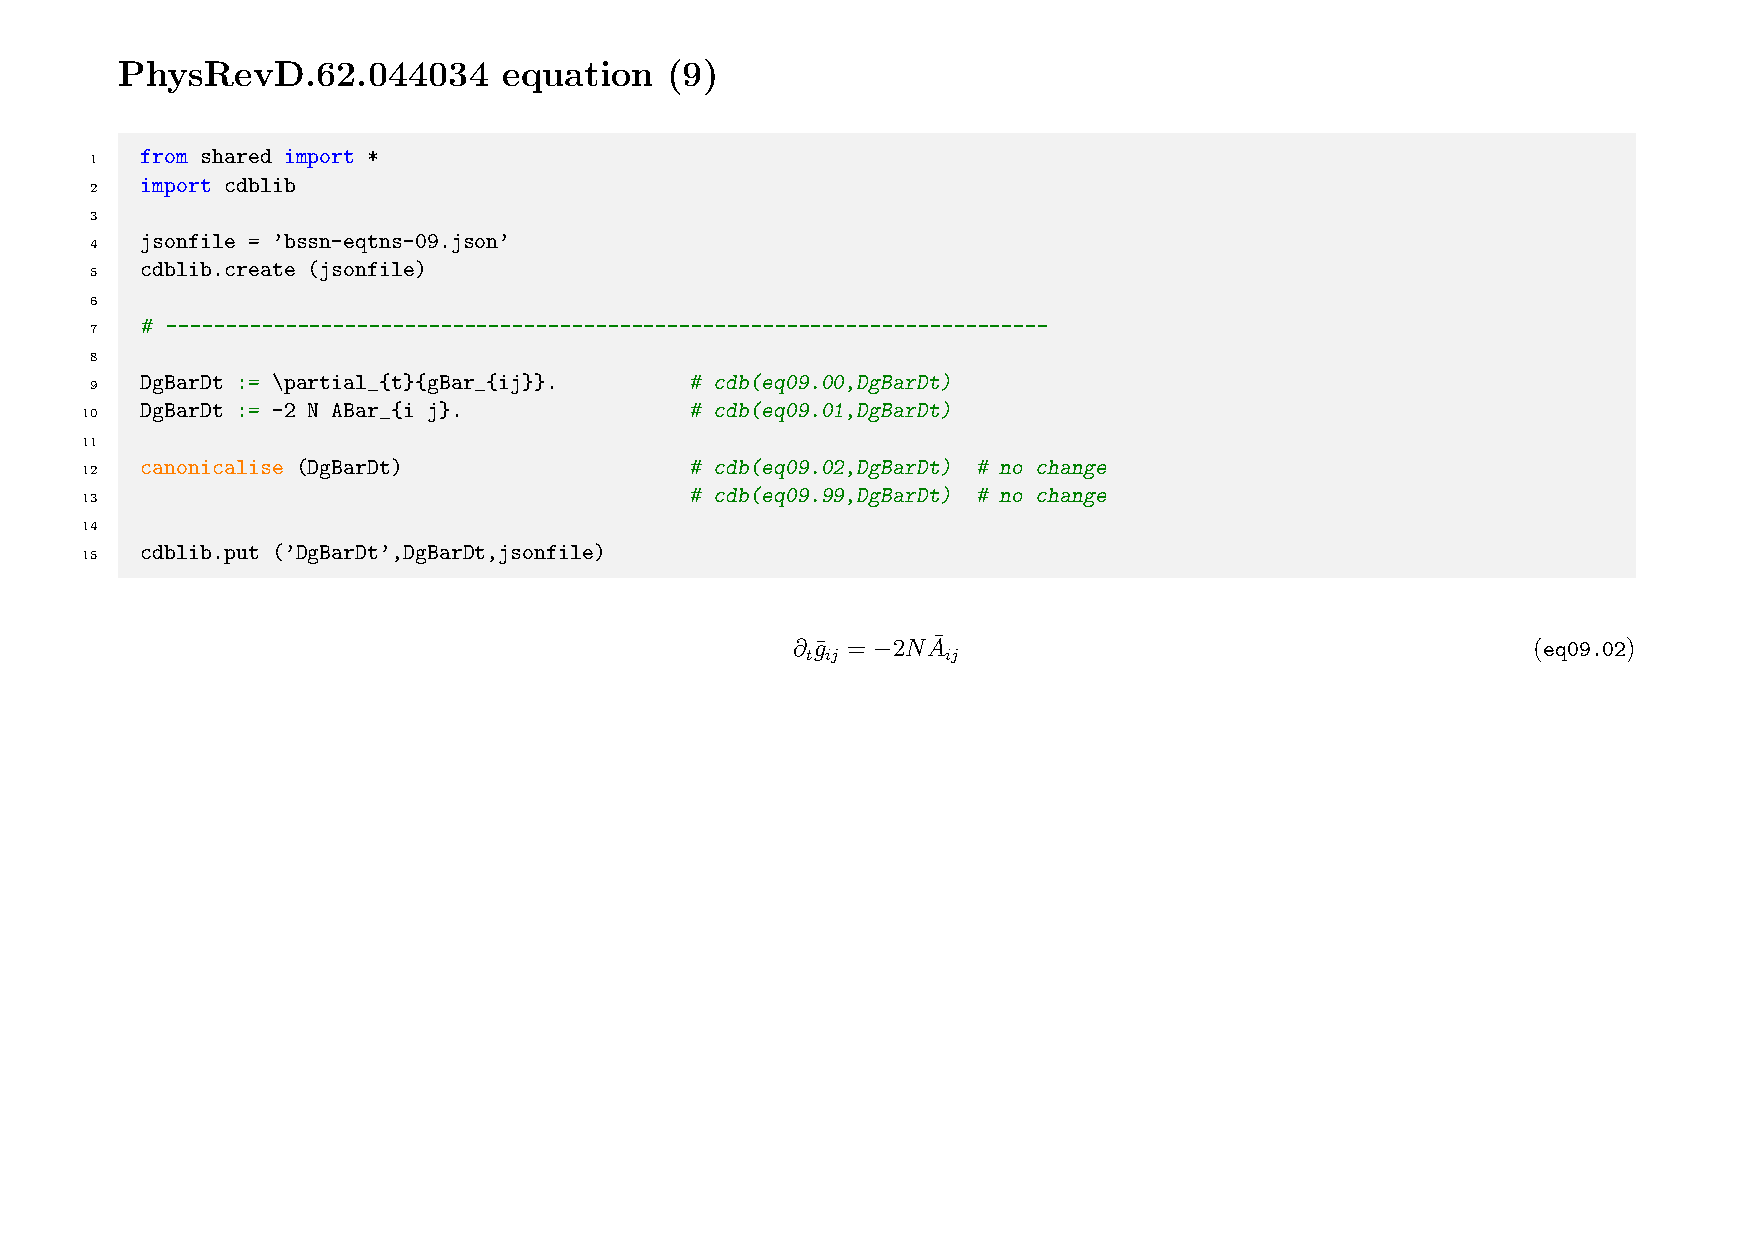
\includepdf[pages=1-]{./bssn-eqtns-09.pdf}
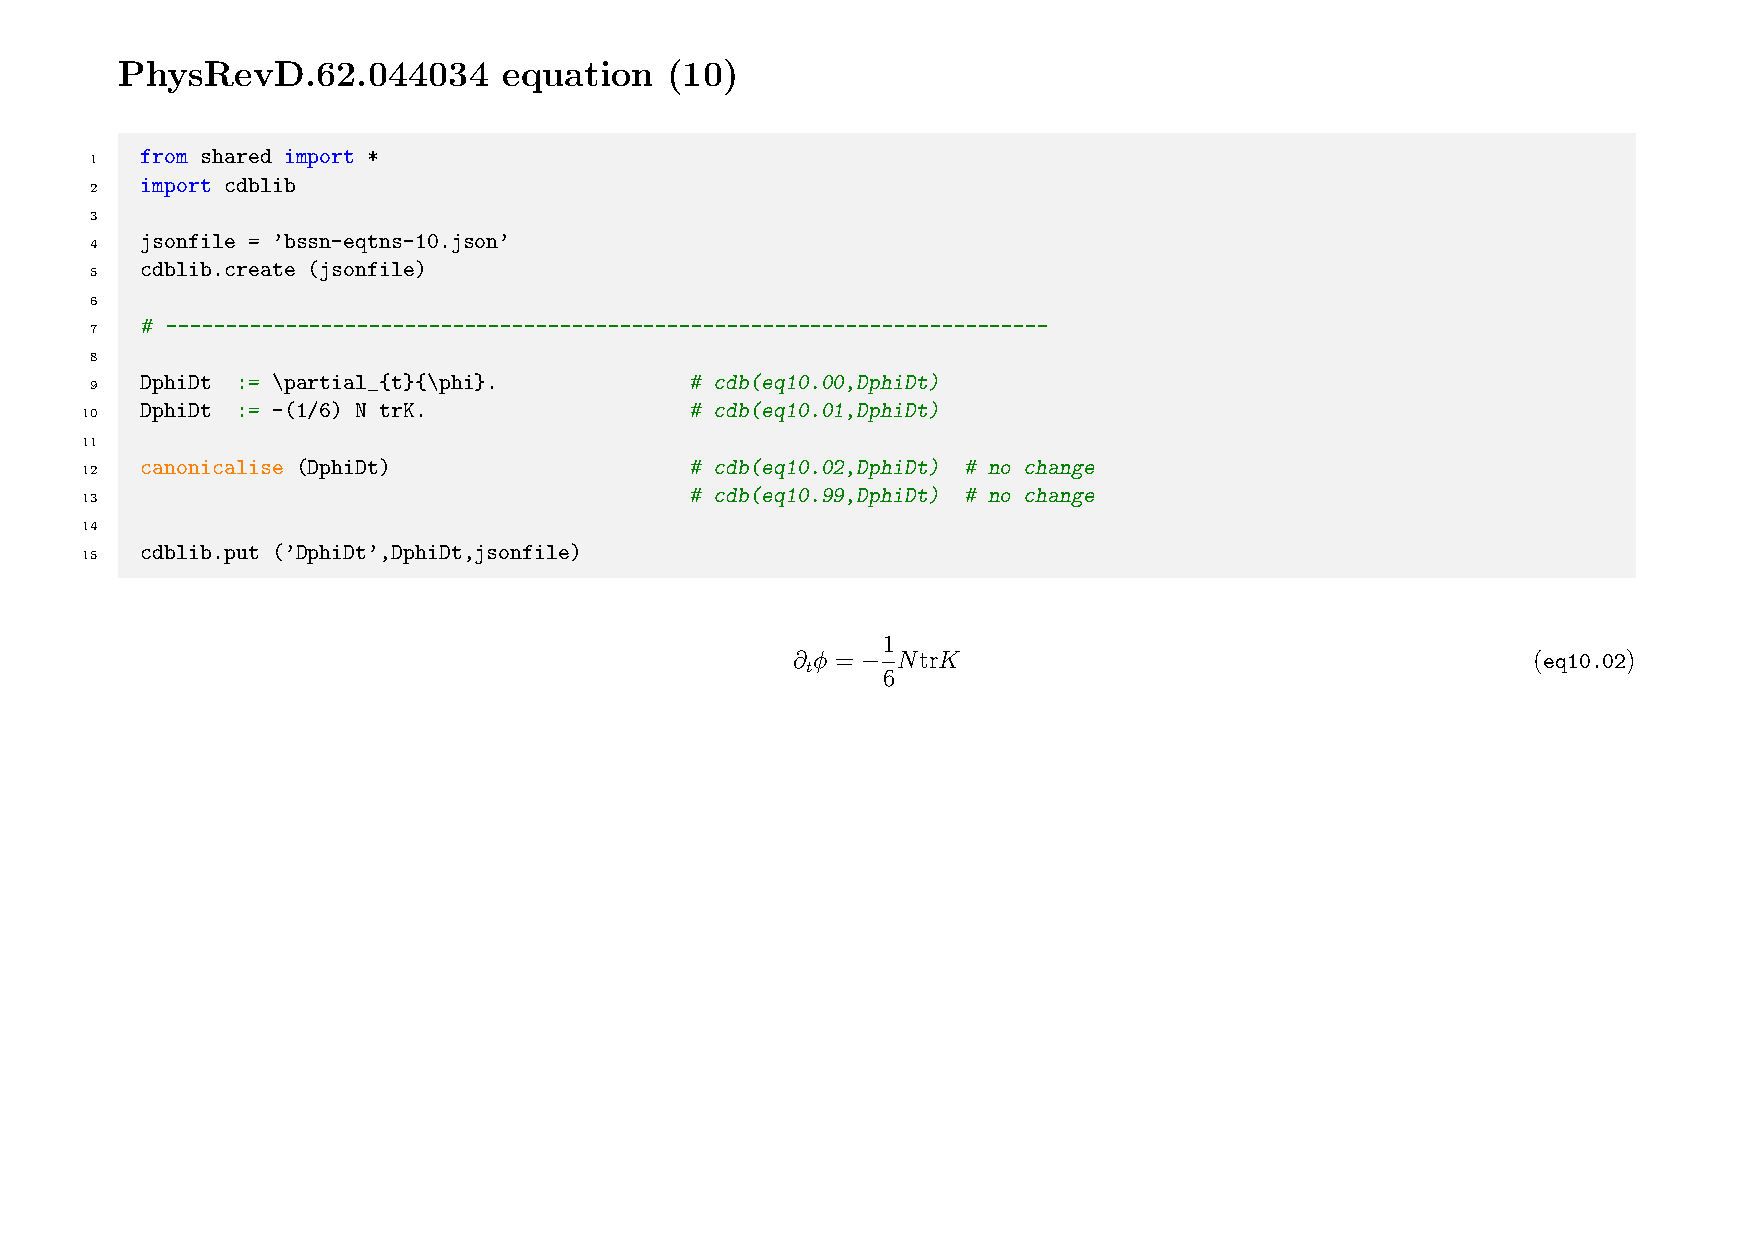
\includepdf[pages=1-]{./bssn-eqtns-10.pdf}
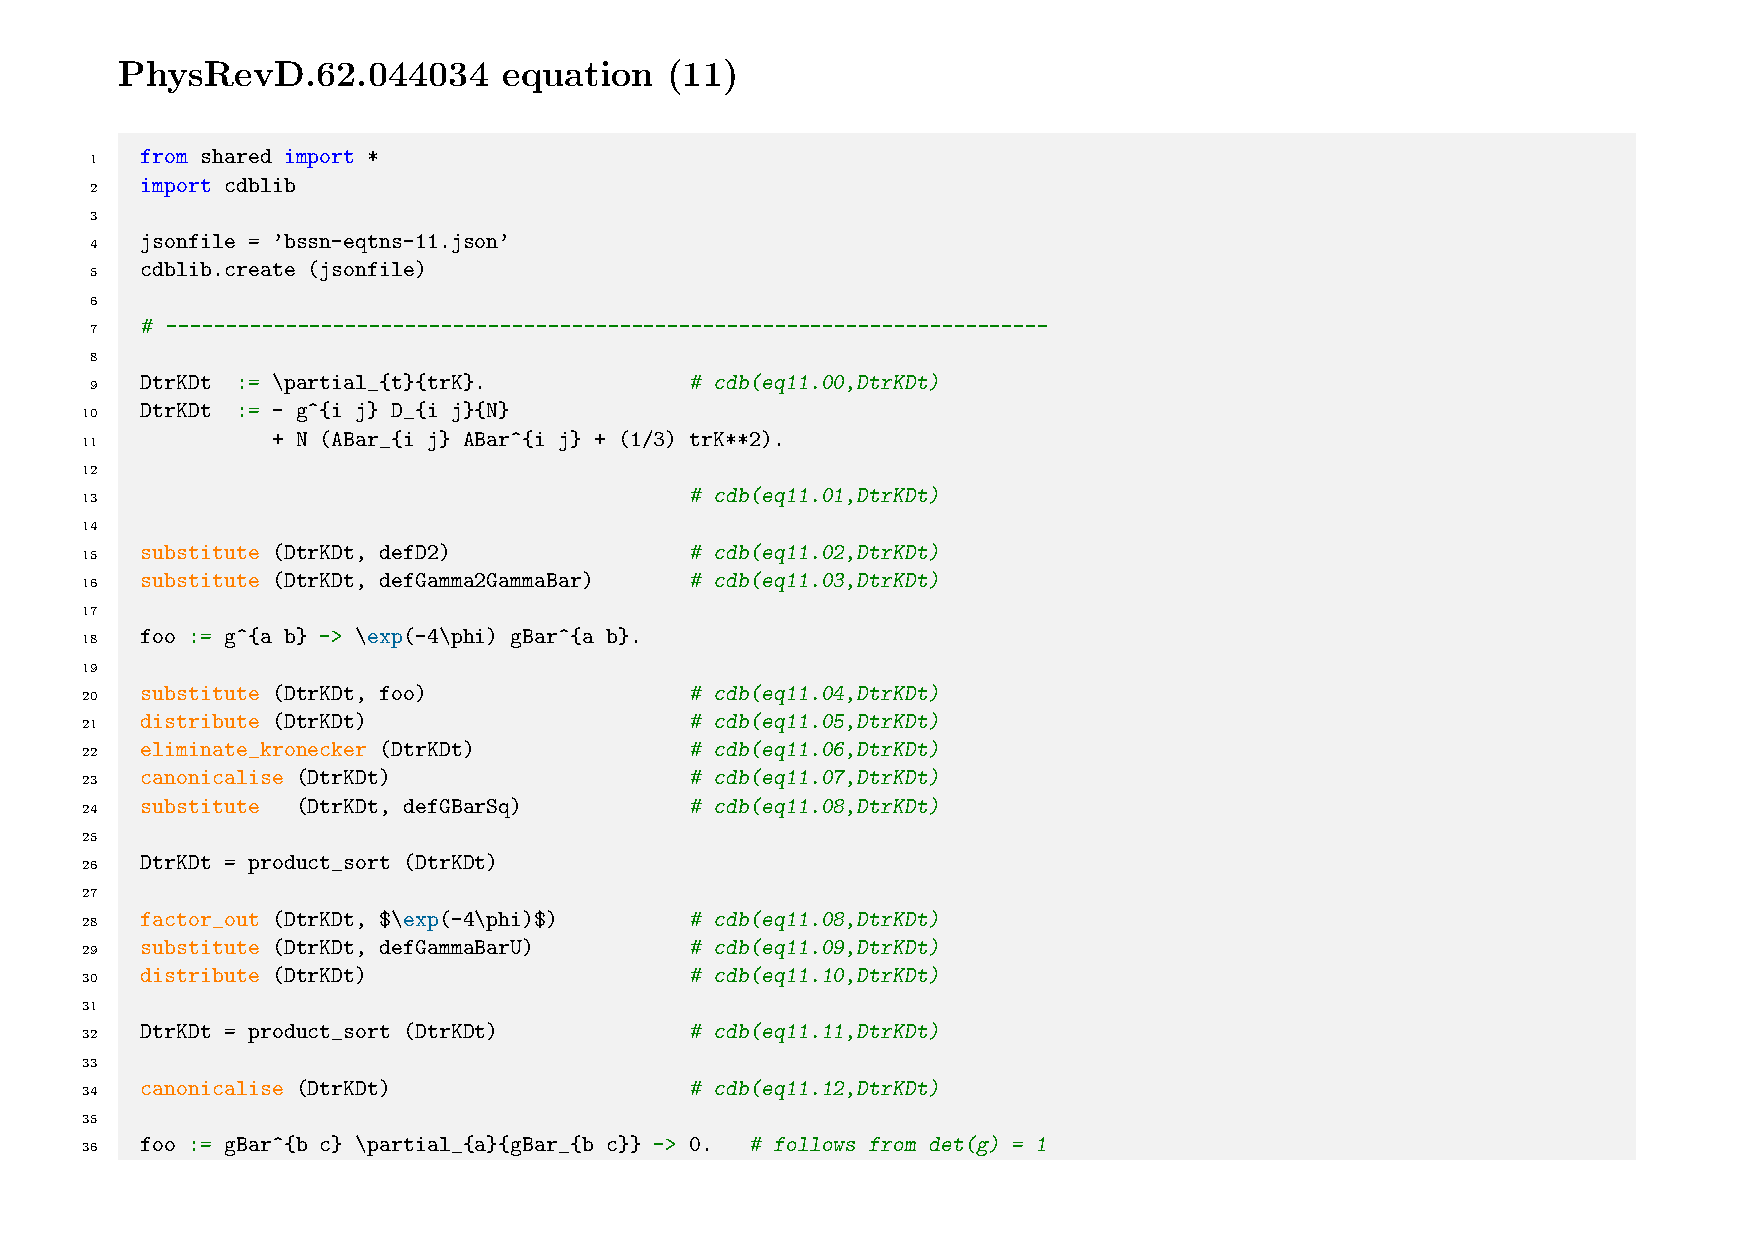
\includepdf[pages=1-]{./bssn-eqtns-11.pdf}
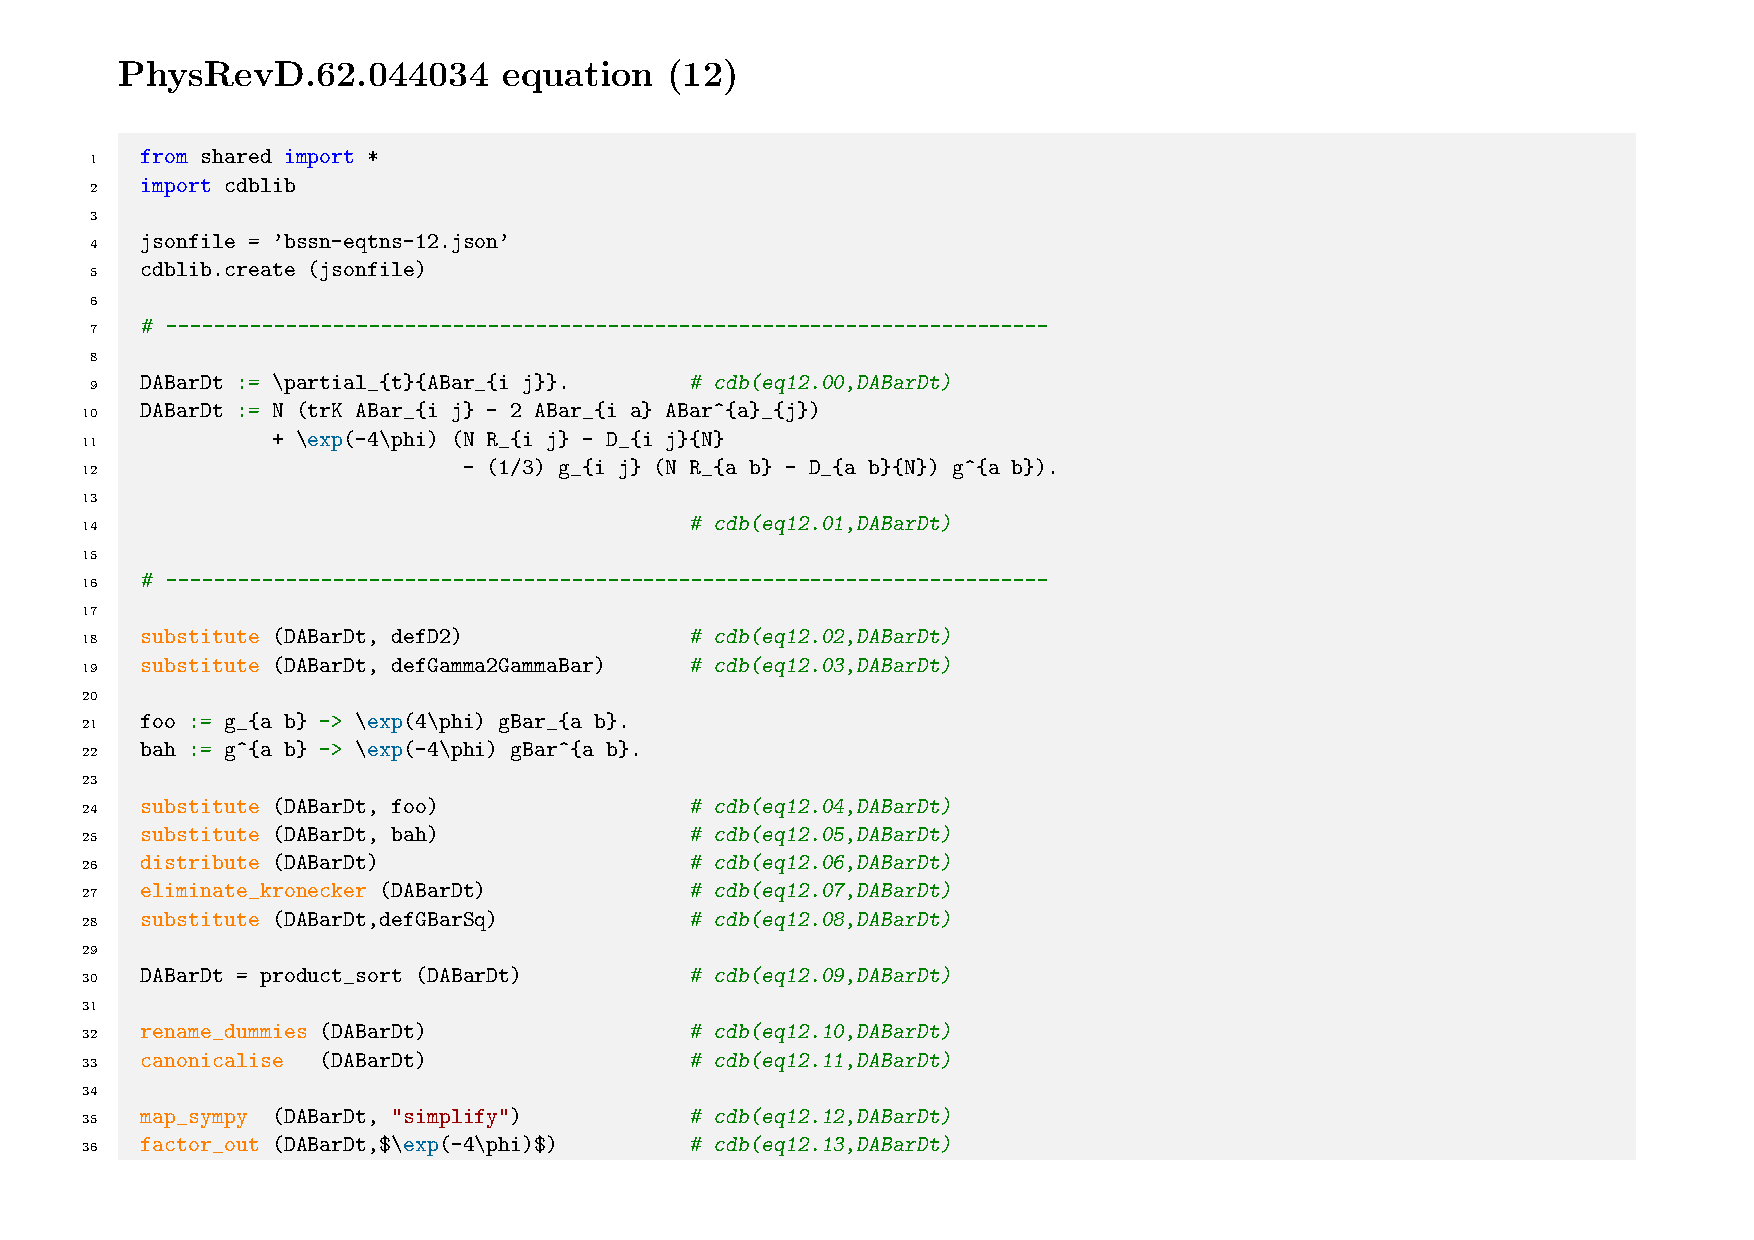
\includepdf[pages=1-]{./bssn-eqtns-12.pdf}
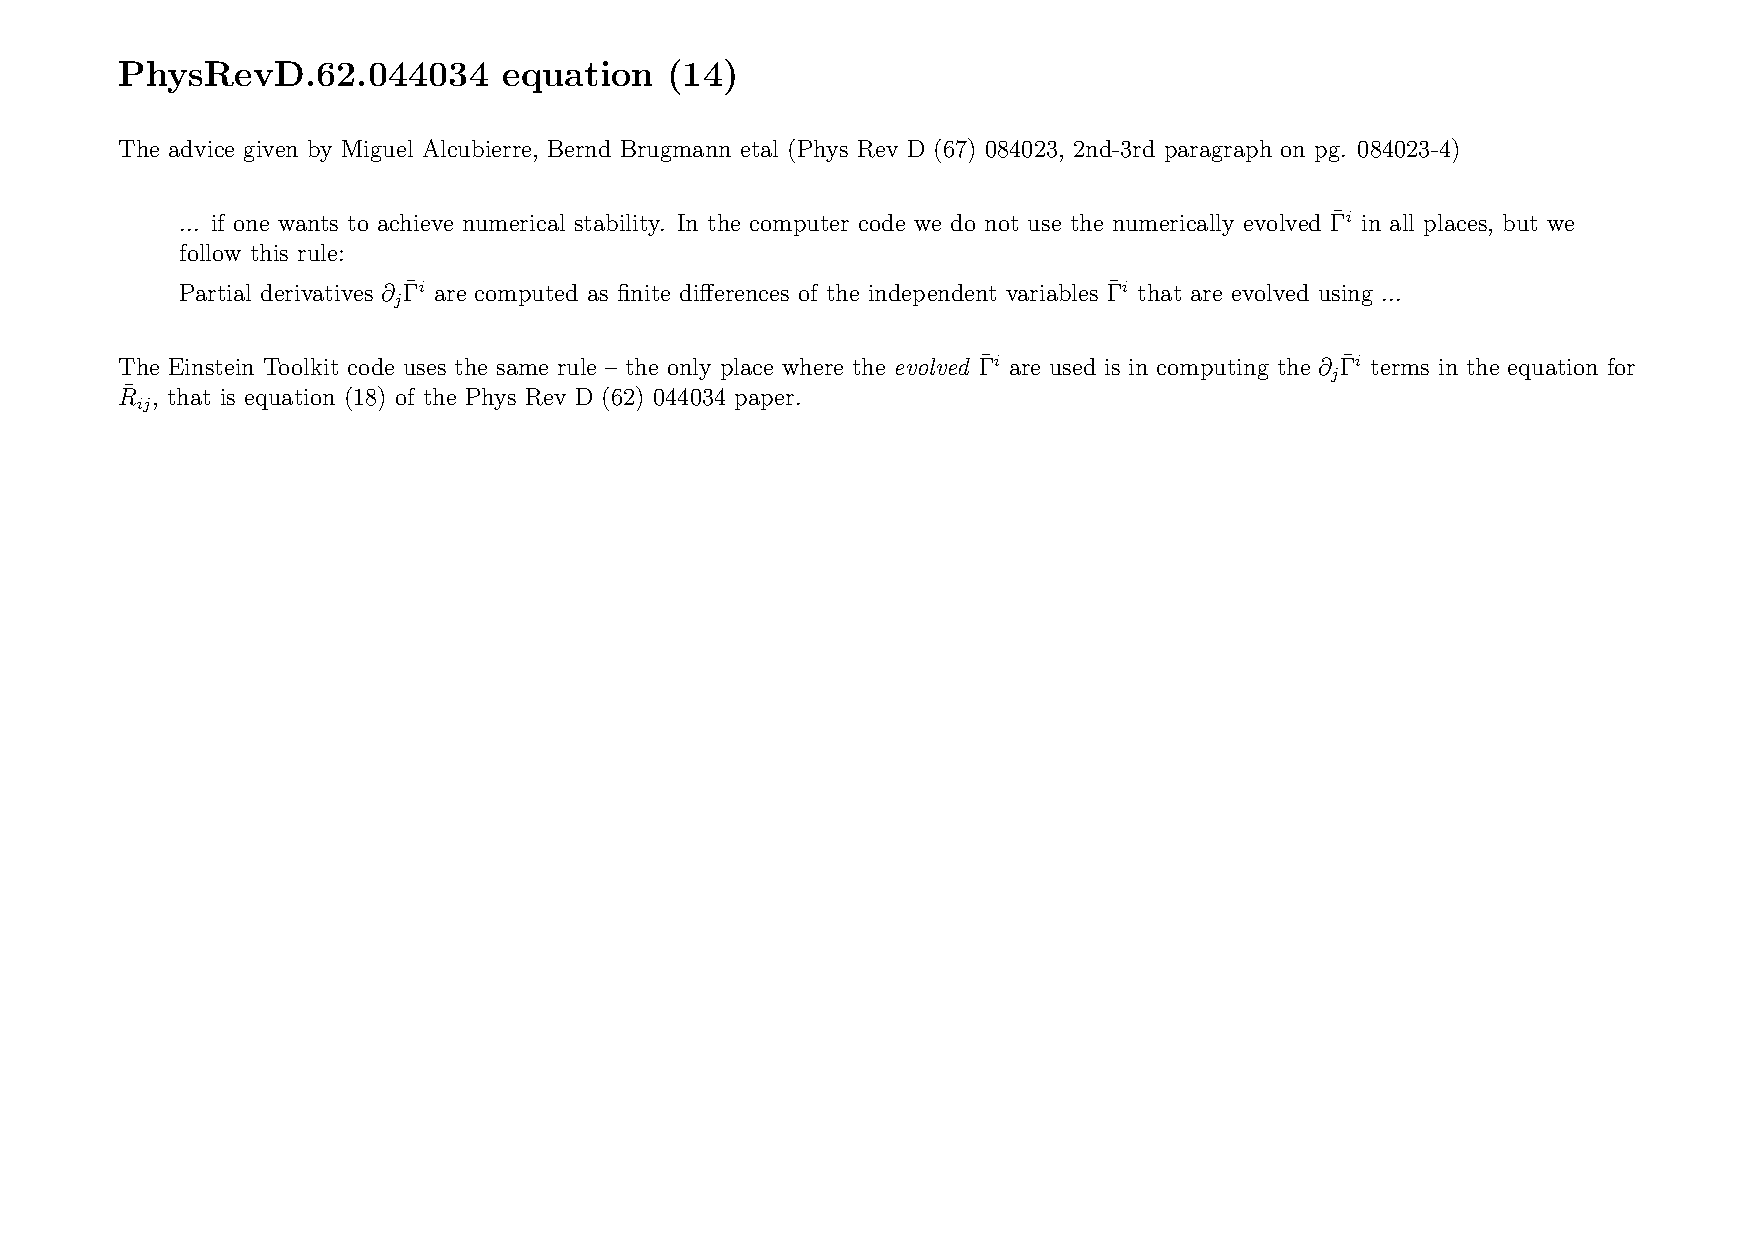
\includepdf[pages=1-]{./bssn-eqtns-14.pdf}
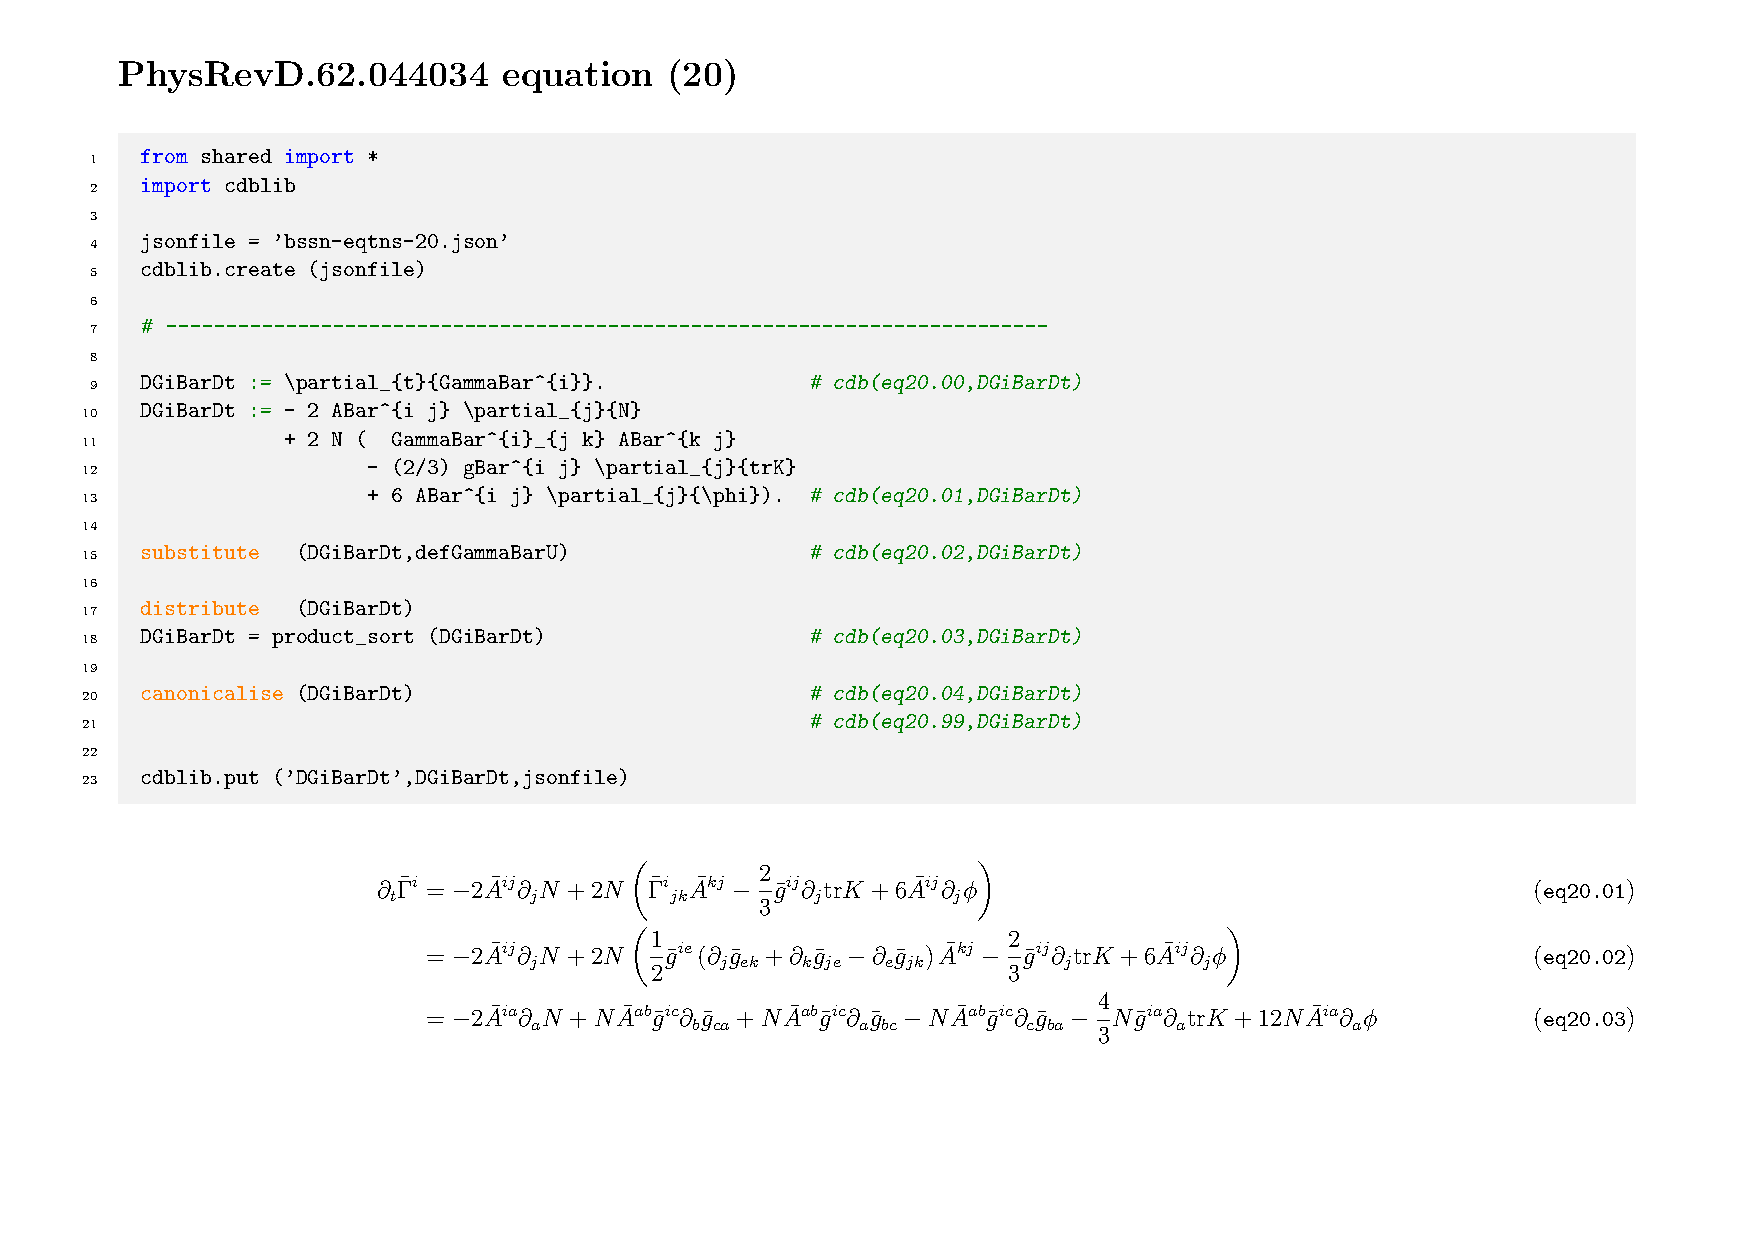
\includepdf[pages=1-]{./bssn-eqtns-20.pdf}
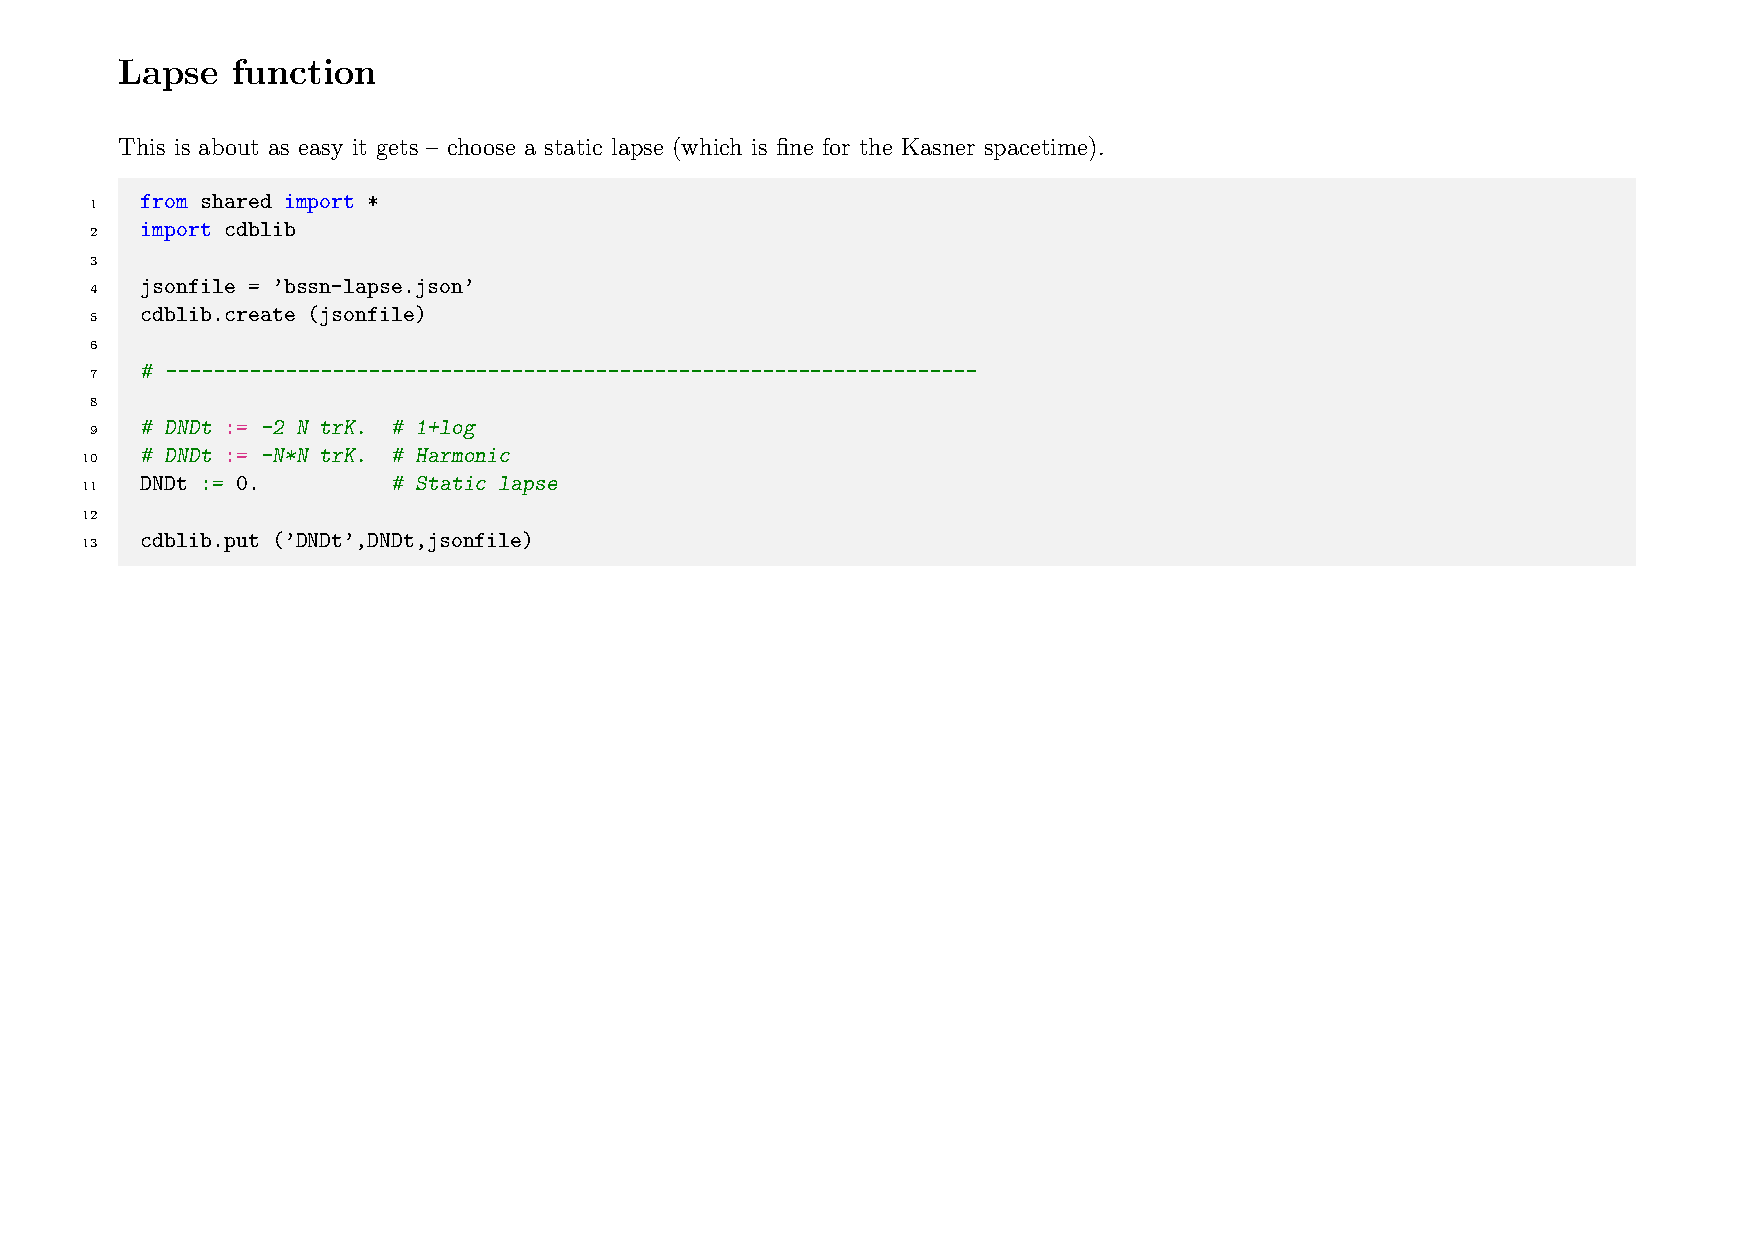
\includepdf[pages=1-]{./bssn-lapse.pdf}
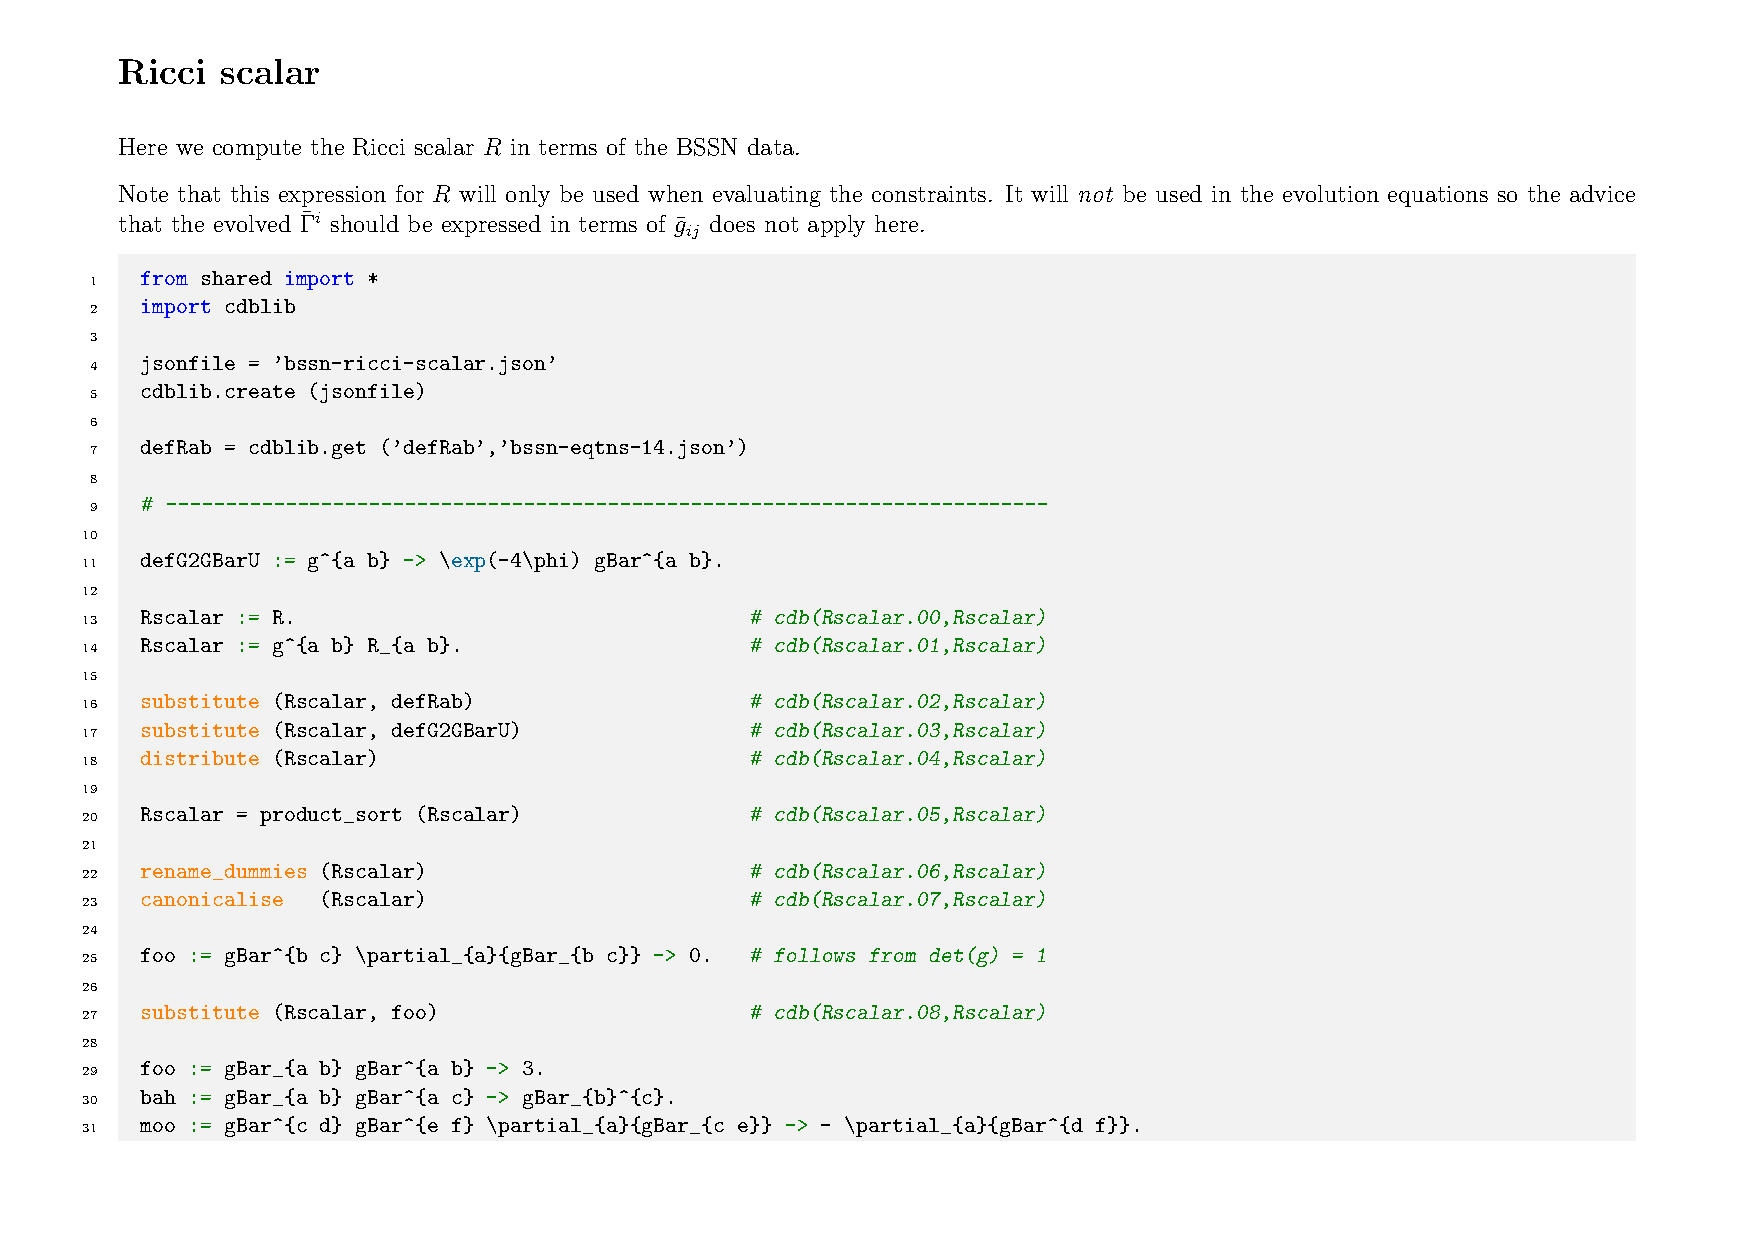
\includepdf[pages=1-]{./bssn-ricci-scalar.pdf}
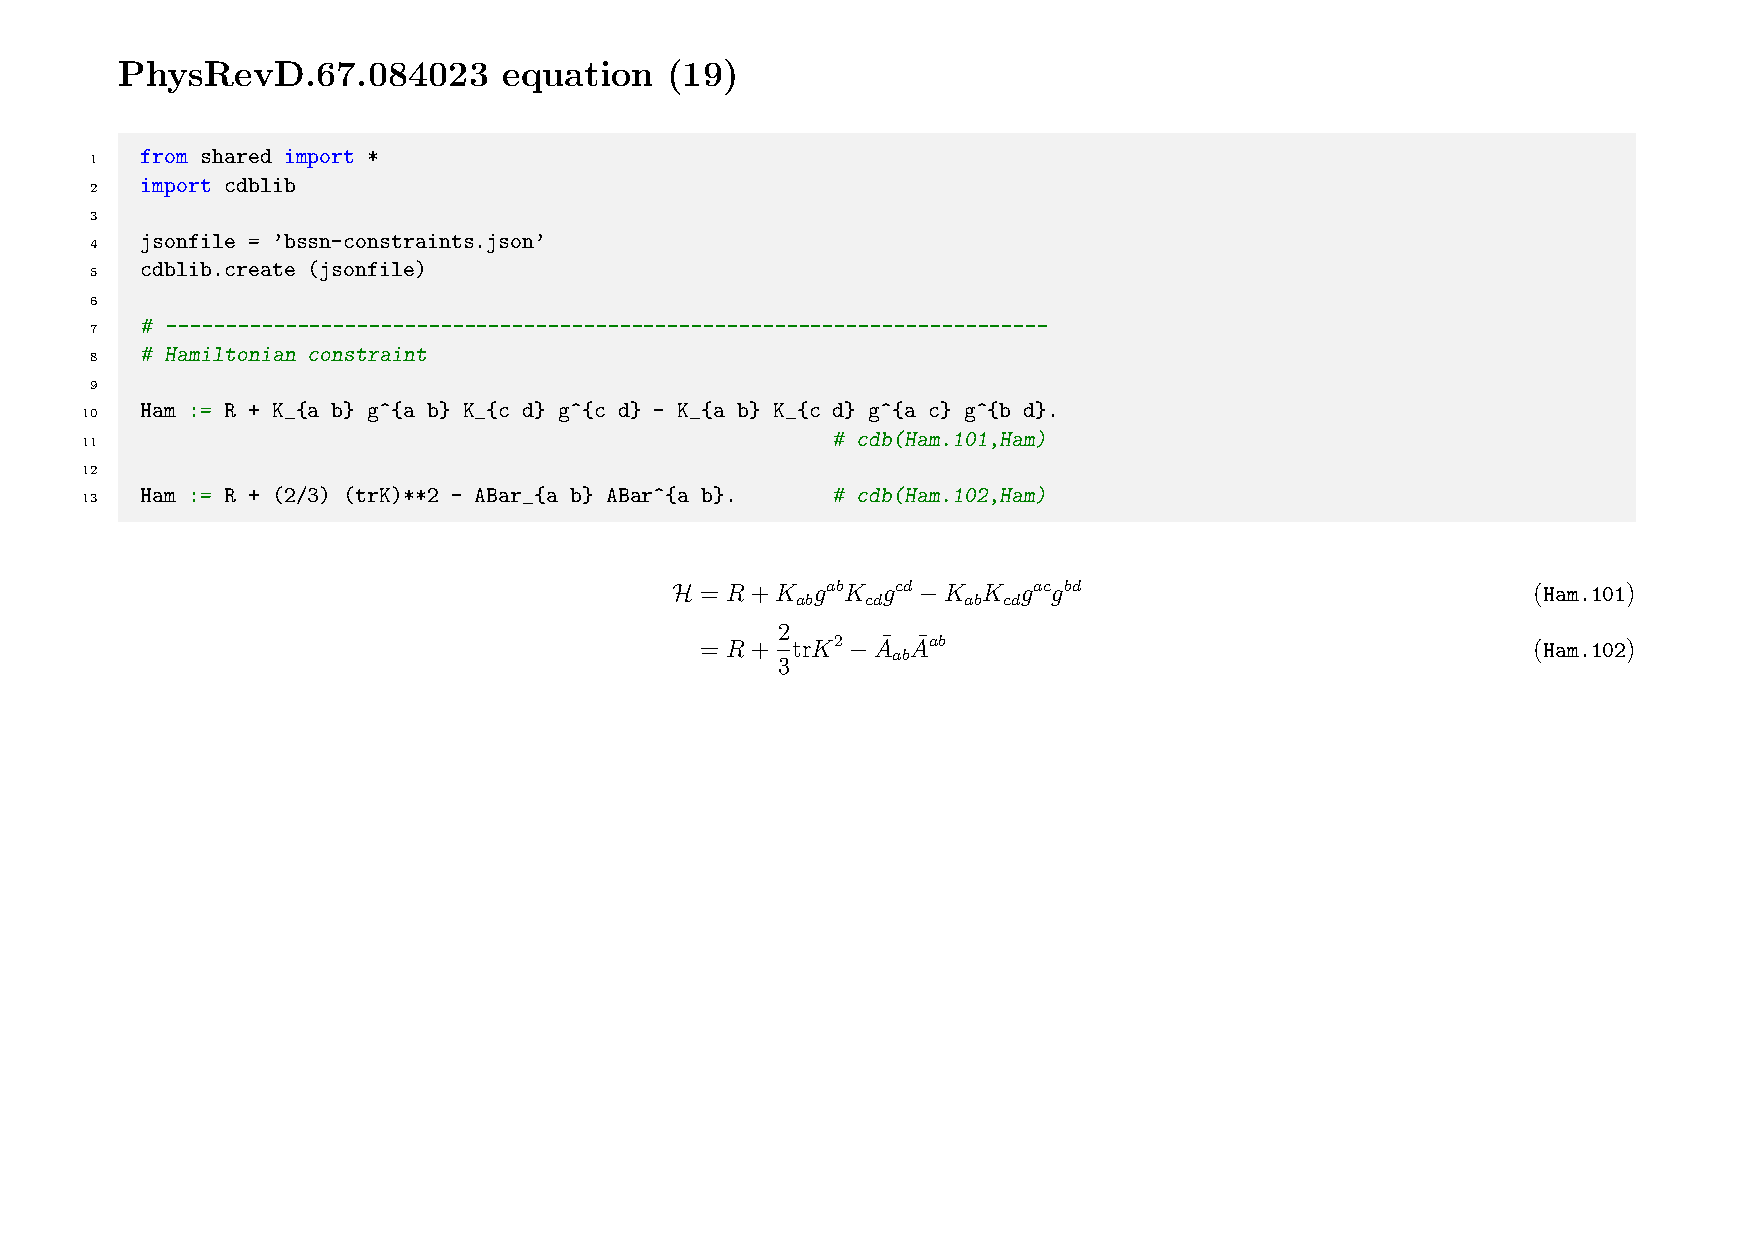
\includepdf[pages=1-]{./bssn-constraints.pdf}

\end{document}
